\chapter{Recherche d’expressions rationnelles}
\label{chap-regexp}

Nous allons voir dans ce chapitre comment rechercher des motifs simples dans un texte
au moyen des expressions rationnelles.

\section{Définition}
\index{Expressions rationnelles}

Le but de ce chapitre n’est pas de faire une introduction aux langages formels, mais
de montrer comment utiliser les expressions rationnelles dans Unitex pour rechercher des
motifs simples. Le lecteur intéressé par une présentation plus formelle pourra se reporter
aux nombreux ouvrages qui traitent du sujet.


\bigskip \noindent Une expression rationnelle peut-être:

\begin{itemize}
  \item une unité lexicale (\verb+livre+) ou un masque lexical
  (\verb+<manger.V>+);
  \item une position particulière du texte : le début \verb+{^}+ou la fin \verb+{$}+
  \item la concaténation de deux expressions rationnelles (\verb+je mange+);\index{Concaténation d'expressions rationnelles}
  \item l'union de deux expressions rationnelles (\verb$Pierre+Paul$);\index{Union d'expressions rationnelles} 
  \item l’étoile de Kleene d’une expression rationnelle (\verb+très*+).\index{Etoile de Kleene}
\end{itemize}


\section{Unités lexicales}
\index{Unité lexicale}

Dans une expression rationnelle, l’unité lexicale a la même définition qu’en \ref{tokenization}
(page \pageref{tokenization}). Notons que les symboles point, plus, étoile, inférieur ainsi que les
parenthèses ouvrantes et fermantes ont une signification particulière, il faut donc les
déspécialiser avec le caractère \verb+\+ si l’on souhaite les rechercher. Voici quelques exemples
d’unités lexicales valides: \index{\verb+\+}

\begin{verbatim}
chat
\.
<N:ms>
{S}
\end{verbatim}

\index{Respect de la casse}
\noindent Par défaut, Unitex tolère que des mots avec des minuscules reconnaissent des mots écrits
avec des majuscules. Il est possible de forcer le respect de la casse en utilisant les guillemets.
Ainsi, \verb+"pierre"+ ne reconnaît que la forme \verb+pierre+ et non pas \verb+Pierre+ ou \verb+PIERRE+.

\bigskip
\noindent NOTE: si l’on souhaite rendre la présence d’un espace obligatoire, il faut le mettre entre
guillemets.

\index{Espace!obligatoire}


\section{Motifs}
\index{Masque!lexical}
Un masque lexical est une requête qui reconnaît une unité lexicale ou une suite d'unités lexicales

\subsection{Symboles spéciaux}
\label{section-special-symbols}
\index{Meta-symbols}

Il y a deux sortes de motifs. La première catégorie regroupe tous les symboles présentés à la
section ~\ref{section-sentence-splitting} à l’exception de \verb$<PNC>$, qui reconnaît des signes de
ponctuation, et du symbole \verb+<^>+, qui reconnaît un retour à ligne. Tous les retours à la ligne
ayant été remplacés par des espaces, ce symbole n’a plus aucune utilité lors de la recherche de
motifs. Ces symboles, également appelés \textit{métas}, sont les suivants:


\bigskip
\index{\verb+<MOT>+}\index{\verb+<MIN>+}\index{\verb+<MAJ>+}\index{\verb+<PRE>+}\index{\verb+<NB>+}
\index{\verb+#+}\index{\verb+<E>+}\index{\verb+<DIC>+}\index{\verb+<SDIC>+}\index{\verb+<CDIC>+}
\index{\verb+<TDIC>+}
\begin{itemize}
  \item \verb+<E>+ : mot vide, ou epsilon. Reconnaît la séquence vide;
  \item \verb+<TOKEN>+ : reconnaît n’importe quelle unité lexicale sauf l'espace
  	  utilisé par défaut pour les filtres morphologiques;
  \item \verb+<MOT>+ : reconnaît n’importe quelle unité lexicale formée de lettres;
  \item \verb+<MIN>+ : reconnaît n’importe quelle unité lexicale formée de lettres minuscules;
  \item \verb+<MAJ>+ : reconnaît n’importe quelle unité lexicale formée de lettres majuscules;
  \item \verb+<PRE>+ : reconnaît n’importe quelle unité lexicale formée de lettres et commençant par
  	  une
majuscule;
  \item \verb+<DIC>+ : reconnaît n’importe quel mot figurant dans les dictionnaires du texte;
  \item \verb+<SDIC>+ : reconnaît n’importe quel mot simple figurant dans les dictionnaires du
  	  texte;
  	  \index{Mots!simples}
  \item \verb+<CDIC>+ : reconnaît n’importe quel mot composé figurant dans les dictionnaires du
  	  texte;
  	  \index{Mots!composés}
  \item \verb+<TDIC>+ : reconnaît n’importe quelle unité lexicale tagguée comme
  	  \verb+{XXX,XXX.XXX}+;
  \item \verb+<NB>+ : reconnaît n’importe quelle suite de chiffres contigus
  	  (1234 est reconnue mais pas 1 234) ;
  \item \verb+#+ : interdit la présence de l'espace.\index{Espace!interdit}
\end{itemize}

\bigskip
\noindent NOTE : comme il a été dit en section \ref{tokenization}, AUCUN des métas ne peut être utilisé pour reconnaître le marqueur \verb+{STOP}+\index{\verb+{STOP}+}, pas même \verb+<TOKEN>+.

\subsection{Masques lexicaux}
\index{Masques lexicaux}\index{Dictionnaires!référence aux}
\index{Dictionnaire!du texte}

La seconde sorte de masques lexicaux regroupe ceux qui font appel aux informations contenues
dans les dictionnaires du texte. Les quatre formes possibles sont :


\bigskip
\begin{itemize}
\item \verb+<lire>+: reconnaît toutes les entrées qui ont \verb+lire+ comme forme canonique.
	On remarque que cette forme est ambiguë si \verb+lire+ est aussi un code grammatical ou
	sémantique;
  \item \verb+<lire.>+: reconnaît toutes les entrées qui ont \verb+lire+ comme forme canonique.
  	  Ce masque lexical n'est pas ambigu avec le précédent;
  \item \verb+<be.V>+: reconnaît toutes les entrées qui ont \verb+lire+ comme forme canonique
                       et qui ont le code grammatical  \verb+V+;
  \item \verb+<V>+: reconnaît toutes les entrées qui ont le code grammatical \verb+V+.
  	  Ce masque lexical est ambigu comme le premier. Pour lever l'ambuguité, on peut utiliser
  	  \verb+<.V>+ ou \verb$<+V>$;
   \index{Etiquettes!lexicales}
\item \verb+{lirons,lire.V}+ ou \verb+<lirons,lire.V>+: reconnaît toutes les entrées qui ont
	\verb+lir-+\newline\verb+ons+ comme forme fléchie, \verb+lire+ comme forme canonique et qui
	ont le code grammatical
  \verb+V+. Ce type de masque n’a d’intérêt que si l’on travaille sur l’automate du texte où sont
  explicitées les ambiguïtés des mots.
  \index{Texte!automate du}\index{Automate!du texte} Lorsque l’on effectue une recherche sur
le texte, ce masque reconnaît la même chose que la simple unité lexicale \verb+lirons+.
\end{itemize}

\subsection{Contraintes grammaticales et sémantiques}

Les masques lexicaux des exemples précédents sont simples. Il est possible d’exprimer des
motifs plus complexes en indiquant plusieurs codes grammaticaux ou sémantiques, séparés
par le caractère \verb$+$. Une entrée de dictionnaire ne sera alors reconnue que si elle 
possède tous les codes présents dans le masque.
 Le masque \verb$<N+z1>$ reconnaît ainsi les entrées :

\bigskip
\noindent
\texttt{broderies,broderie.N+z1:fp}

\noindent
\texttt{capitales europ\'eennes,capitale europ\'eenne.N+NA+Conc+HumColl+z1:fp}

\bigskip
\noindent mais pas:

\bigskip
\noindent
\texttt{Descartes,Ren\'e Descartes.N+Hum+NPropre:ms}

\noindent
\texttt{habitu\'e,.A+z1:ms}

\bigskip
\noindent Il est possible d’exclure des codes en les faisant précéder du caractère \verb+~+
au lieu de \verb$+$. Pour être reconnue, une entrée doit contenir tous les codes autorisés par le
masque et aucun des codes interdits. \verb$<A~z3>$ reconnaît tous les adjectifs qui n'ont pas le
code \verb+z3+ (cf. table~\ref{tab-semantic-codes}). Si vous voulez faire référence à un code
contenant le caractère \verb$~$ vous devez le déspécialiser en le faisant précéder d'un \verb+\+.

\bigskip
\noindent REMARQUE: Avant la version 2.1, l'opérateur de négation était le signe moins. Si l'on veut
uiliser d'anciens graphes, sans les modifier, il faut appeler \verb+Locate+ en ligne de commande
avec l'option \verb+-g minus+.
                       
\index{Exclusion des codes grammaticaux et sémantiques}\index{\verb+~+}

\bigskip
\noindent L’ordre dans lequel les codes apparaissent dans le masque n’a aucune importance. Les
trois masques lexicaux suivants sont équivalents :


\begin{verbatim}
<N~Hum+z1>
<z1+N~Hum>
<~Hum+z1+N>
\end{verbatim}

\bigskip
\noindent NOTE: il n’est pas possible d’utiliser un masque n’ayant que des codes d'interdiction.
\verb+<~N>+ et \verb+<~A~z1>+ sont donc des masques incorrects.
Il est toutefois possible d’exprimer de telles contraintes en utilisant des contextes (voir section
~\ref{section-contexts}).



\subsection{Contraintes flexionnelles}
\index{Contraintes flexionnelles}
On peut également spécifier des contraintes portant sur les codes flexionnels. Ces contraintes
doivent obligatoirement être précédées par au moins un code grammatical ou sémantique. Elles se
présentent comme les codes flexionnels présents dans les dictionnaires. Voici quelques exemples de
masques lexicaux utilisant des contraintes flexionnelles :

\bigskip
\begin{itemize}
  \item \verb+<A:m>+ reconnaît un adjectif au masculin;
  \item \verb+<A:mp:f>+ reconnaît un adjectif qui est, soit au masculin pluriel, soit au féminin;
  \item \verb+<V:2:3>+ reconnaît un verbe à la 2\ieme ou 3\ieme personne ; cela exclut tous les
  temps qui n’ont ni 2\ieme ni 3\ieme personne (infinitif, participe passé, et participe présent)
  ainsi que les temps conjugués à la première personne.

\end{itemize}

\bigskip
\noindent Pour qu’une entrée de dictionnaire $E$ soit reconnue par un masque $M$, il faut qu’au
moins un code flexionnel de $E$ contienne tous les caractères d’un code flexionnel de $M$.
Considérons l’exemple suivant :

\bigskip
$E$=\verb$sépare,séparer.V:W:P1s:P3s:S1s:S3s:Y2s$

$M$=\verb$<V:P2s:Y2s>$

\bigskip
\noindent Aucun code flexionnel de $E$ ne contient à la fois les caractères \verb+P+, \verb+2+ et
\verb+s+. Cependant, le code \verb+Y2s+ de $E$ contient bien les caractères \verb+Y+ et \verb+2+. Le
code \verb+Y2+ est inclus dans au moins un code de $E$, le masque lexical $M$ reconnaît donc l’entrée $E$. L’ordre des caractères à l’intérieur d’un code flexionnel est sans importance.


\subsection{Négation d’un motif}
\index{Négation d’un motif}
\index{\verb+"!+}
Il est possible de faire la négation d’un motif au moyen du caractère~\verb+!+ placé immédiatement
après le caractère ~\verb+<+. La négation est possible sur les métas \verb+<MOT>+, \verb+<MIN>+,
\verb+<MAJ>+, \verb+<PRE>+, \verb+<DIC>+  ainsi que sur les masques lexicaux ne comportant que des
codes grammaticaux, sémantiques ou flexionnels (\textit{i.e.} \verb$<!V~z3:P3>$). Les motifs
\verb+#+ et \verb+" "+  sont la négation l’un de l’autre.
\index{Negation}\index{\verb+<E>+}\index{\verb+<NB>+}\index{\verb+#+}
Le méta \verb$<!MOT>$ peut reconnaître toutes les unités lexicales qui ne sont pas formées de
lettres, sauf le séparateur de phrases \verb+{S}+ et, bien sûr, le marqueur \verb+{STOP}+.
La négation est sans effet sur \verb+<NB>+, \verb+<SDIC>+, \verb+<CDIC>+, \verb+<TDIC>+ et
\verb+<TOKEN>+.

\bigskip
\noindent La négation est interprétée d’une façon particulière dans les métas 
\verb+<!DIC>+, \verb+<!MIN>+, \verb+<!MAJ>+ et \verb+<!PRE>+.
\index{\verb+<DIC>+}\index{\verb+<MIN>+}\index{\verb+<MAJ>+}\index{\verb+<PRE>+}
Au lieu de reconnaître toutes les formes qui ne sont pas reconnues
par le méta sans la négation, ces motifs ne donnent que des formes qui sont des séquences
de lettres. Ainsi, le méta \verb+<!DIC>+ permet d’obtenir les mots inconnus du texte. Ces formes
inconnues sont le plus souvent des noms propres, des néologismes et des fautes d’orthographe.


\bigskip
\noindent La négation d’un masque lexical comme  \verb+<V:G>+ reconnaît tous les mots sauf ceux qui
peuvent être reconnus par ce masque. Ainsi, le masque \verb+<!V:G>+ ne reconnaîtra pas la forme
anglaise being, même s’il existe dans les dictionnaires du texte des entrées non verbales pour ce
mot:



\begin{verbatim}
being,.A
being,.N+Abst:s
being,.N+Hum:s
\end{verbatim}
\index{Mots!inconnus}

\bigskip
\begin{figure}[h]
\begin{center}
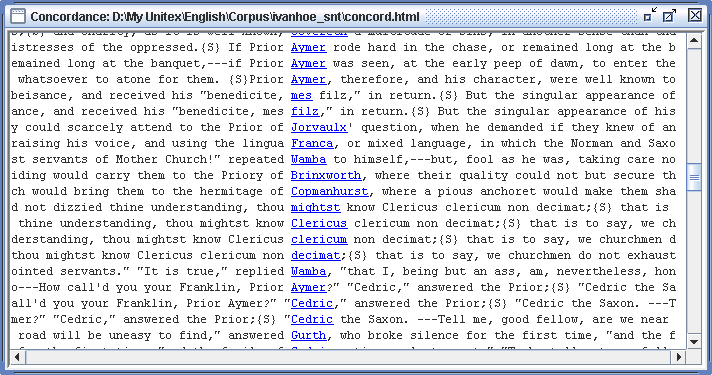
\includegraphics[width=15cm]{resources/img/fig4-1.png}
\caption{Résultat de la recherche du méta \texttt{<!DIC>}}
\end{center}
\end{figure}

\bigskip
\noindent Voici plusieurs exemples de motifs mélangeant les différentes sortes de contraintes:

\begin{itemize}
  \item \verb$<A~Hum:fs>$ : adjectif non humain au féminin singulier;
  \item \verb+<lire.V:P:F>+ : le verbe \textit{lire} au présent ou au futur;
  \item \verb$<suis,suivre.V>$ : le mot \textit{suis} en tant que forme conjuguée du verbe
  	  \textit{suivre}
  	  (par opposition à la forme du verbe \textit{être});
  \item \verb$<facteur.N~Hum>$ : toutes les entrées nominales ayant \textit{facteur} comme forme
  	  canonique et ne possédant pas le code sémantique \verb+Hum+;
  \item \verb$<!ADV>$ : tous les mots qui ne sont pas des adverbes;
  \item \verb$<!MOT>$ : tous les caractères, qui ne sont pas des lettres, sauf le séparateur de
  	  phrases
  	  (voir figure~\ref{fig-search-<!MOT>}). Ce masque ne reconnait pas le séparateur de phrase
  	  \verb+{S}+
  	  ni le tag \verb+{STOP}+.
  	  \index{\verb+{S}+}\index{Séparateur de phrase}\index{\verb+{STOP}+}
\end{itemize}

\bigskip
\begin{figure}[h]
\begin{center}
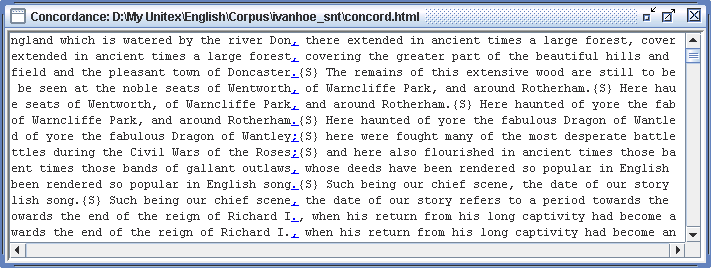
\includegraphics[width=15cm]{resources/img/fig4-2.png}
\caption{Résultat de la recherche du méta
\texttt{<!MOT>}\label{fig-search-<!MOT>}}
\end{center}
\end{figure}

\section{Concaténation}
\index{Concaténation d'expressions rationnelles}\index{\verb+.+}\index{Opérateur!concaténation}

On peut concaténer des expressions rationnelles de trois façons. La première consiste à
utiliser l’opérateur de concaténation représenté par le point. Ainsi, l’expression:

\begin{verbatim}
<DET>.<N>
\end{verbatim}

\noindent reconnaît un déterminant suivi par un nom. L’espace peut également servir à concaténer.
L’expression de l’exemple suivant:


\begin{verbatim}
le <A> chat
le<A>chat
\end{verbatim}

\noindent reconnaît l’unité lexicale \textit{le}, suivie d’un adjectif et de l’unité lexicale \textit{chat}.
Les parenthèses \index{Parenthèses} servent à délimiter une expression rationnelle.
Toutes les expressions suivantes sont équivalentes:


\begin{verbatim}
le <A> chat
(le <A>)chat
le.<A>chat
(le).<A> chat
(le.(<A>)) (chat)
\end{verbatim}

\section{Union}
\index{Union d'expressions rationnelles}\index{\verb$+$}
\index{Opérateur!disjonction}
L’union d’expressions rationnelles se fait en les séparant par le caractère \verb$+$.
L’expression:

\begin{verbatim}
(je+tu+il+elle+on+nous+vous+ils+elles) <V>
\end{verbatim}

\noindent
reconnaît un pronom suivi par un verbe. Si l’on veut rendre un élément facultatif dans
une expression, il suffit de faire l’union de cet élément avec le mot vide epsilon.
\index{\verb+<E>+} Exemples:

\bigskip
\noindent \verb$le(petit+<E>)chat$ reconnaît les séquences \textit{le chat}
et \textit{le petit chat}

\smallskip
\noindent \verb$(<E>+franco-)(anglais+belge)$ reconnaît \textit{anglais}, \textit{belge},
\textit{franco-anglais} et \textit{franco-belge}

\section{Kleene star}
\index{Kleene star}\index{\verb+*+}\index{Opérateur!Kleene star}
L’étoile de Kleene, représentée par le caractère \verb+*+,permet de reconnaître zéro, une ou
plusieurs occurrences d’une expression. L’étoile doit être placée à droite de l’élément concerné.
L’expression :


\begin{verbatim}
il fait très* froid
\end{verbatim}

\noindent reconnaît \textit{il fait froid}, \textit{il fait très froid},
\textit{il fait très très froid}, etc. L’étoile est prioritaire sur les
autres opérateurs. Il faut utiliser les parenthèses pour appliquer l’étoile à une expression
complexe. L’expression :


\begin{verbatim}
0,(0+1+2+3+4+5+6+7+8+9)*
\end{verbatim}

\noindent reconnaît un zéro, suivie d’une virgule et d’une suite éventuellement vide de chiffres.

\bigskip
\noindent ATTENTION : il est interdit de rechercher le mot vide avec une expression rationnelle.
Si l’on essaye de chercher \verb$(0+1+2+3+4+5+6+7+8+9)*$, le programme signalera une erreur
comme le montre la figure~\ref{fig-epsilon-error}.


\bigskip
\begin{figure}[h]
\begin{center}
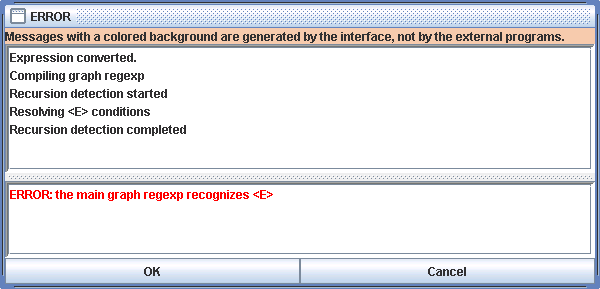
\includegraphics[width=14cm]{resources/img/fig4-3.png}
\caption{Erreur lors de la recherche d’une expression reconnaissant le mot vide \label{fig-epsilon-error}}
\end{center}
\end{figure}


\section{Filtres morphologiques}
\label{section-filters}
\index{Filtres morphologiques}

Il est possible d’appliquer des filtres morphologiques aux unités lexicales recherchées.
Pour cela, il faut faire suivre immédiatement l’unité lexicale considérée par un filtre entre
doubles angles:


\bigskip
\noindent
\textit{motif}\verb$<<$\textit{motif morphologique}\verb$>>$ \\


\bigskip\index{Expressions régulières}\index{POSIX}
\noindent Les filtres morphologiques s’expriment sous la forme d’expressions régulières au format
POSIX (voir \cite{TRE} pour une syntaxe détaillée). Voici quelques exemples de filtres élémentaires:




\begin{itemize}
  \item \verb$<<ss>>$: contient \verb$ss$
  \item \verb$<<^a>>$: commence par \verb$a$
  \item \verb+<<ez$>>+: finit par \verb$ez$
  \item \verb$<<a.s>>$: contient \verb$a$ suivi par un caractère quelconque, suivi par \verb$s$
  \item \verb$<<a.*s>>$: contient \verb$a$ suivi par un nombre de caractères quelconque, suivi par \verb$s$
  \item \verb$<<ss|tt>>$: contient \verb$ss$ ou \verb$tt$
  \item \verb$<<[aeiouy]>>$: contient une voyelle non accentuée
  \item \verb$<<[aeiouy]{3,5}>>$: contient une séquence de voyelles non accentuées, de longueur comprise entre 3 et 5
  \item \verb$<<es?>>$: contient \verb$e$ fsuivi par un \verb$s$ facultatif
  \item \verb$<<ss[^e]?>>$: contient \verb$ss$ suivi par un caractère qui n’est pas une voyelle \verb$e$
\end{itemize}

\bigskip
\noindent Il est possible de combiner ces filtres élémentaires pour former des filtres plus complexes:

\begin{itemize}
\item \verb+<<[ai]ble$>>+: finit par \verb$able$ ou \verb$ible$
\item \verb$<<^(anti|pro)-?>>$: commence par \verb$anti$ ou \verb$pro$, suivi par un tiret facultatif
  \item \verb+<<^([rst][aeiouy]){2,}$>>+: mot formé de 2 ou plus séquences commençant par un 
  	\verb$r$, \verb$s$ ou \verb$t$ suivi d’une voyelle non accentuée
  \item \verb!<<^([^l]|l[^e])>>!: ne commence pas par \verb$l$ ou alors la deuxième lettre n’est pas
un \verb$e$, c’est-à-dire n’importe quel mot sauf ceux qui commencent par \verb$le$.                                                                           De telles contraintes peuvent être exprimées plus simplement en utilisant des contextes
(voir~\ref{section-contexts}).
\end{itemize}

\noindent Par défaut, un filtre morphologique tout seul est considéré comme s’appliquant au méta
\verb$<TOKEN>$, c’est-à-dire à n’importe quelle unité lexicale sauf l’espace et le marqueur
\verb+{STOP}+.
En revanche, lorsqu’un filtre suit immédiatement un motif, il s’applique à ce qui est reconnu par
le motif. Voici quelques exemples de telles combinaisons:


\begin{itemize}
  \item \verb+<V:K><<i$>>+: participe passé finissant par \verb$i$
  \item \verb!<CDIC><<->>!: mot composé contenant un tiret
  \item \verb!<CDIC><< .* >>!: mot composé contenant deux espaces
  \item \verb!<A:fs><<^pro>>!: adjectif féminin singulier commençant par \verb$pro$
  \item \verb!<DET><<^([^u]|(u[^n])|(un.+))>>!: déterminant différent de \verb$un$
  \item \verb+<!DIC><<es$>>+: mot qui n’est pas dans le dictionnaire et qui se termine par \verb$es$
  \item \verb!<V:S:T><<uiss>>!: verbe au subjonctif passé ou présent, contenant \verb$uiss$
\end{itemize}

\noindent \index{Respect de la casse}NOTE : par défaut, les filtres morphologiques sont soumis aux
même variations de casse que les masques lexicaux. Ainsi, le filtre \verb$<<^é>>$ va reconnaître
tous les mots commençant par \texttt{é,}, mais également ceux qui commencent par \texttt{E} ou 
\texttt{É}. 
Pour forcer le respect exact de la casse du filtre, il faut ajouter \verb+_f_+ immédiatement après
celui-ci. Exemple : \verb+<A><<^é>>_f_+.



\section{Recherche}
\index{Configuration de la recherche}
\subsection{Configuration de la recherche}
Pour pouvoir rechercher une expression, il faut tout d’abord ouvrir un texte (voir chapitre
~\ref{chap-text}). Cliquez ensuite sur "Locate Pattern..." dans le menu "Text". La fenêtre de la
figure~\ref{fig-regexp-search-configuration} apparaît alors.

\bigskip
\begin{figure}[h]
\begin{center}
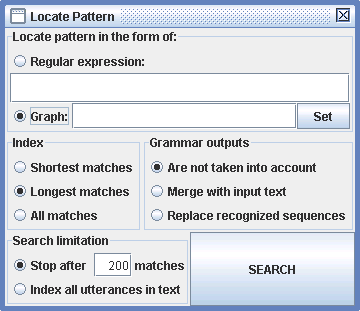
\includegraphics[width=8.8cm]{resources/img/fig4-4.png}
\caption{Fenêtre de recherche d’expressions\label{fig-regexp-search-configuration}}
\end{center}
\end{figure}

\noindent Le cadre "Locate Pattern" permet de choisir entre une expression rationnelle et une
grammaire. Cliquez sur "Regular expression".


\bigskip
\noindent Le cadre "Index" permet de sélectionner le mode de reconnaissance:

\bigskip
\index{Shortest matches}\index{Longest matches}\index{All matches}
\begin{itemize}
  \item "Shortest matches" : donne la priorité aux séquences les plus courtes
  	  %For instance, if your grammar can recognize the sequences \textit{a very hot chili} and 
  %\textit{very hot}, the first one will be discarded;
  \item "Longest matches" : donne la priorité aux séquences les plus longues. C’est le mode utilisé
  	  par défaut;
  \item "All matches" : donne toutes les séquences reconnues.
\end{itemize}

\bigskip
\noindent Le cadre "Search limitation" permet de limiter ou non la recherche à un certain nombre
d’occurrences. Par défaut, la recherche est limitée aux 200 premières occurrences.
\index{Occurrences!nombre}

\bigskip
\noindent Les options du cadre "Grammar outputs" ne concernent pas les expressions rationnelles.
Elles sont décrites à la section
~\ref{section-applying-graphs-to-text}. De même pour les options de l'onglet
"Advanced options" (voir section \ref{section-advanced-search-options}).

\bigskip
\noindent Dans le cadre "Search algorithm", on définit si l'on veut effectuer la recherche dans le
texte avec le programme \verb+Locate+ ou dans l'automate du texte avec le programme \verb+LocateTfst+.
Par défaut la recherche est effectuée avec le programme \verb+Locate+. Pour utiliser
\verb+LocateTfst+, il est utile de se référer à la section \ref{section-locate-tfst}.

\bigskip
\noindent Entrez une expression et cliquez sur "Search" pour lancer la recherche. Unitex va transformer
l’expression en une grammaire au format \verb+.grf+.
\index{Fichier!\verb+.grf+} Cette grammaire va ensuite être compilée en une grammaire au format
\verb+.fst2+\index{Fichier!\verb+.fst2+} qui sera utilisée par le programme de recherche.


\subsection{Affichage des résultats}
\label{section-display-occurrences}
Une fois la recherche terminée, la fenêtre de la figure~\ref{fig-search-results}
apparaît, indiquant le nombre d’occurrences trouvées, le nombre d’unités lexicales reconnues,
ainsi que le rapport entre ce nombre et le nombre total d’unités lexicales du texte.

\bigskip
\begin{figure}[h]
\begin{center}
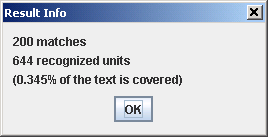
\includegraphics[width=6.5cm]{resources/img/fig4-5.png}
\caption{Résultats de la recherche \label{fig-search-results}}
\end{center}
\end{figure}

\noindent Après avoir cliqué sur "OK", vous verrez apparaître la fenêtre de la
figure~\ref{fig-configuration-concordance} permettant de configurer l’affichage de la liste
des occurrences trouvées. Vous pouvez également faire apparaître cette fenêtre en cliquant sur
"Display Located Sequences..." dans le menu "Text".
On appelle \textit{concordance}\index{Concordance} la liste d’occurrences.


\bigskip
\begin{figure}[h]
\begin{center}
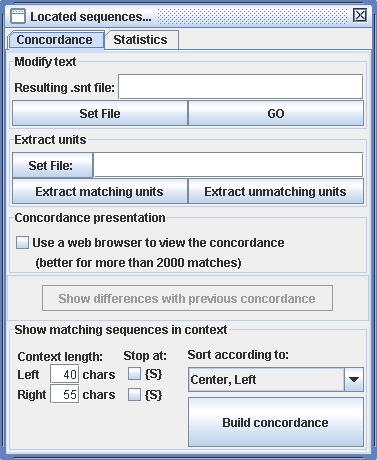
\includegraphics[width=11cm]{resources/img/fig4-6.png}
\caption{Configuration de l’affichage des occurrences trouvées\label{fig-configuration-concordance}}
\end{center}
\end{figure}

\bigskip
\noindent Le cadre "Modify text" offre la possibilité de remplacer les occurrences trouvées par les
sorties produites. Cette possibilité sera examinée au chapitre
~\ref{chap-advanced-grammars}.

\bigskip
\noindent Le cadre "Extract units" vous permet de construire un fichier texte avec toutes les phrases
contenant ou non des occurrences. Le bouton "Set File" vous permet de sélectionner le fichier
de sortie. Cliquez ensuite sur "Extract matching units" ou "Extract unmatching units" selon
que vous voulez extraire les phrases contenant les occurrences ou non.


\bigskip
\noindent Dans le cadre "Show Matching Sequences in Context", vous pouvez sélectionner la
longueur en caractères des contextes gauche et droit des occurrences qui seront affichées dans
la concordance. Si une occurrence a une longueur inférieure à la taille du contexte droit, la
ligne de concordance sera complétée avec le nombre de caractères nécessaire. Si une occurrence 
a une longueur supérieure à la taille du contexte droit, elle est affichée en entier.


\bigskip
\noindent NOTE: en thaï, la taille des contextes est mesurée en caractères affichables et non en
caractères réels. Cela permet de conserver l’alignement des lignes de concordance malgré la
présence de caractères diacritiques qui se combinent à d’autres lettres au lieu de s’afficher
comme des caractères normaux.


\index{Tri!des concordances}
\index{Contextes!concordance}
\bigskip
\noindent Vous pouvez sélectionner le mode de tri à appliquer dans la liste "Sort According to". Le
mode "Text Order" affiche les occurrences dans l’ordre où elles apparaissent dans le texte.
Les six autres modes permettent de trier en colonnes. Les trois zones d’une ligne sont le
contexte gauche, l’occurrence et le contexte droit. Les occurrences et les contextes droits
sont triés de gauche à droite. Les contextes gauches sont triés de droite à gauche. Le mode
utilisé par défaut est "Center, Left Col.". La concordance est produite sous la forme d’un
fichier HTML.\index{Fichier!HTML}

\bigskip
\noindent Lorsque les concordances atteignent plusieurs milliers d’occurrences, il est préférable
de les afficher avec un navigateur web (Firefox \cite{Firefox}, Netscape \cite{Netscape}, 
Internet Explorer, etc.).\index{Web browser}
\newline
Pour cela, cochez la case "Use a web browser to view the concordance" (voir figure
	~\ref{fig-configuration-concordance}). 
Cette option est activée par défaut lorsque le nombre d’occurrences est supérieur à 3000.
Pour définir le navigateur qui sera utilisé, cliquez sur "Preferences..." dans le menu "Info".
Cliquez sur l’onglet "Text Presentation" et sélectionnez le programme à utiliser dans le cadre
"Html Viewer" (voir figure~\ref{fig-browser-selection}).

\bigskip
\noindent \index{Cadre des concordance} Si vous choisissez d’ouvrir la concordance à l’intérieur
d’Unitex, vous verrez une fenêtre
comme celle de la figure \ref{fig-example-concordance}. 
L’option "Enable links" activée par défaut permet de considérer les occurrences comme des liens
hypertextes.
Ainsi, quand on clique sur une occurrence,
cela ouvre la fenêtre du texte et y sélectionne la séquence reconnue. De plus, si l’automate
du texte est construit et que cette fenêtre n’est pas réduite sous forme d’icône, l’automate
de la phrase contenant l’occurrence cliquée est chargé. Si l’on sélectionne l’option "Allow
concordance edition", on ne peut pas cliquer ainsi sur les occurrences, mais on peut éditer
la concordance comme du texte. Cela permet entre autres de s’y déplacer avec un curseur,
ce qui peut être pratique si l’on travaille sur une concordance avec de grands contextes.


\bigskip
\begin{figure}[h]
\begin{center}
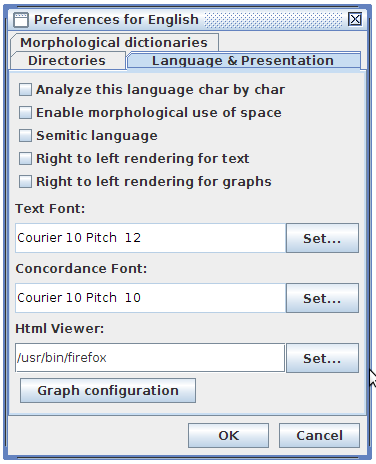
\includegraphics[width=8cm]{resources/img/fig4-7.png}
\caption{Sélection d’un navigateur pour l’affichage des concordances\label{fig-browser-selection}}
\end{center}
\end{figure}

\bigskip
\begin{figure}[!p]
\begin{center}
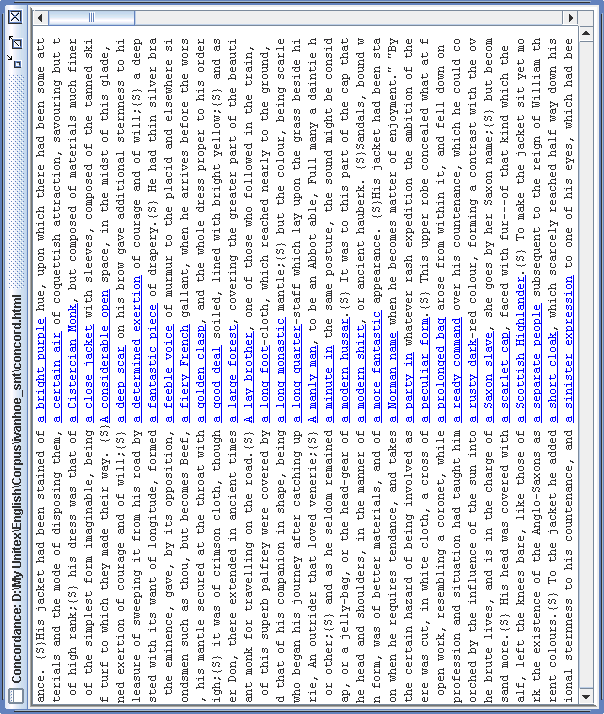
\includegraphics[height=18cm]{resources/img/fig4-8.png}
\caption{Exemple de concordance\label{fig-example-concordance}}
\end{center}
\end{figure}

\clearpage
\subsection{Statistiques}
\label{section-statistics}
Si l'on sélectionne l'onglet ``Statistics'' dans le cadre ``Located sequences..'',
le panneau de la figure~\ref{fig-statistics} apparaît. Ce panneau permet d'effectuer des calculs
statistiques sur les séquences préalablement indexées.

\bigskip
\begin{figure}[!h]
\begin{center}
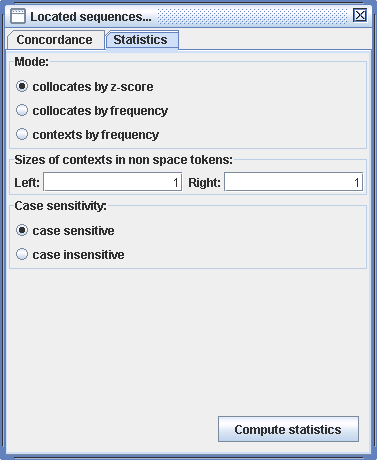
\includegraphics[width=11cm]{resources/img/fig4-9.png}
\caption{Panneau statistiques \label{fig-statistics}}
\end{center}
\end{figure}

\bigskip
\noindent Dans le panneau ``Mode'' il est possible de choisir le type de statistiques désiré:
\begin{itemize}
  \item collocates by frequency: montre les unités lexicales présentes dans le contexte de la
  	  séquence reconnu.
  \item collocates by z-score: le me mêmes informations avec, en plus (number of occurrences of the collocate in the match context and
  in the whole corpus, z-score of the collocate)
  \item contexts by frequency: montre les unités lexicales avec les contextes gauche et droit
  	  (voir au dessous). ``count'' est le nombre d'occurrences d'une séquence reconnue donnée
  	  (munie de contexte)
\end{itemize}

\bigskip
\noindent Dans le second panneau, on choisit la longueur des contextes gauche et droit à utiliser en
tokens sans espace.
NOTE: Cette notion de contexte n'a rien à voir avec celle utilisée dans les grammaires.


\bigskip
\noindent Dans le dernier panneau, on peut permettre ou non la variation de casse.
Si cette variation est permise, \verb$the$ et \verb$THE$ sont considérées comme la même unité
lexicale, et le résultat est la somme de ceux obtenus pour \verb$the$ et \verb$THE$.

\bigskip
\noindent Les figures suivantes montrent les statistiques calculées pour chaque mode pour la requête
\verb$<have>$ sur \verb$ivanhoe.snt$.


\bigskip
\begin{figure}[!h]
\begin{center}
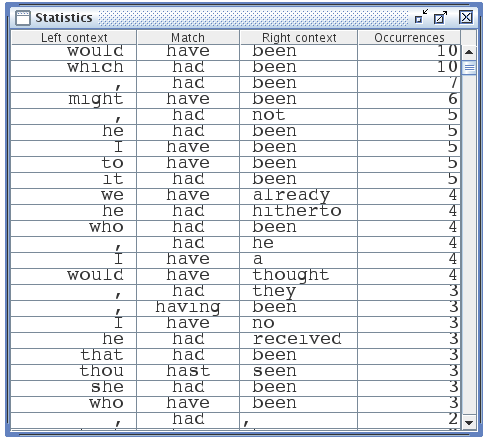
\includegraphics[width=11cm]{resources/img/fig4-10.png}
\caption{contexte gauche+match+contexte droit+nombre d'occurrence\label{fig-statistics-mode0}}
\end{center}
\end{figure}

\begin{figure}[!h]
\begin{center}
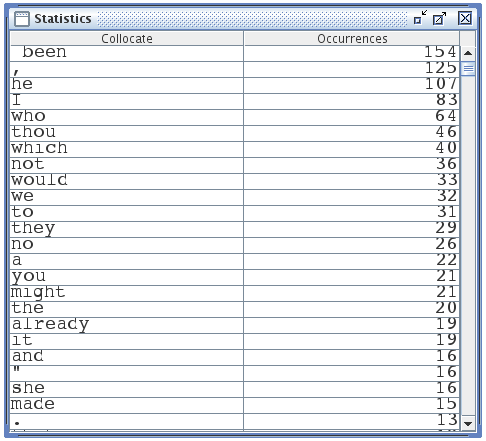
\includegraphics[width=11cm]{resources/img/fig4-11.png}
\caption{collocate count\label{fig-statistics-mode1}}
\end{center}
\end{figure}

\begin{figure}[!h]
\begin{center}
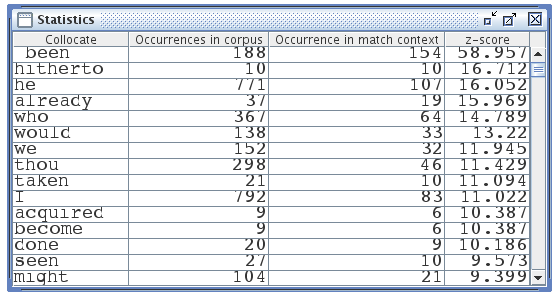
\includegraphics[width=12cm]{resources/img/fig4-12.png}
\caption{collocate, count et d'autres informations\label{fig-statistics-mode2}}
\end{center}
\end{figure}
